\documentclass[10pt,conference,compsocconf]{IEEEtran}

%\usepackage{times}
%\usepackage{balance}
\usepackage{url}
\usepackage{graphicx}	% For figure environment
\usepackage{color}
\usepackage{subcaption}

\newcommand{\todo}[1]{{\color{red}{\textbf{TODO: #1}}}}


\begin{document}
\title{Road Extraction from Aerial Images}
\author{
  Delio Vicini, Matej Hamas, Taivo Pungas\\
  Department of Computer Science, ETH Zurich, Switzerland
}

\maketitle

\begin{abstract}
  TODO - last
\end{abstract}

\section{Introduction}
\label{sec:intro}

The main goal of this paper is to present a novel technique for detecting roads on aerial images. The solution to this problem has potentially many application ranging from automation of map making to urban planning and environmental monitoring.

Given an RGB aerial or satellite image of a moderate resolution (in order of hundreds), we seek to classify each 16x16 patch as \textit{road} or \textit{non-road}. Hence, this is an instance of a binary classification problem.

\begin{figure}[h]
	\centering
	\begin{subfigure}{.2\textwidth}
		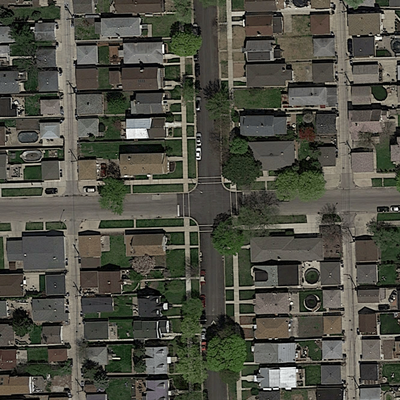
\includegraphics[width=1\textwidth]{figs/img1.png}
	\end{subfigure}
	\begin{subfigure}{.2\textwidth}
		
\includegraphics[width=1\textwidth]{figs/groundtruth1.png}
	\end{subfigure}
	\caption{Aerial image of an urban scene and the ground truth showing the road.}
\end{figure}

As this is quite canonical problem in computer vision, and thanks to its many applications, there is rich previous work in this area \cite{Huang.2002} \cite{MnihThesis.2013} \cite{Long.2014} \cite{Montoya.2015} \cite{Saito.2015}. Most of the past work concentrated on per pixel prediction from aerial images. Some papers also look at multi-class semantic classification by introducing specific \textit{building} class \cite{Saito.2015}. 

Previous approaches include SVMs on manually extracted features \cite{Huang.2002}, convolutional neural networks (CNNs) \cite{Long.2014} \cite{Saito.2015}, conditional random fields \cite{Montoya.2015} and other probabilistic approaches.

Unlike the most of past work, we concentrate on per-patch and not on per-pixel prediction. We have developed a novel solution by combining deep CNN with various post-processing techniques such as dictionary filtering or SVM classification.

Simple 2-layer CNN provides a good starting point for patch classification.  However, the results are noisy. Hence, we modify the CNN architecture, make it deeper and dependant on larger context. Afterwards, we apply various denoising techniques to improve the final prediction. 

We evaluate our algorithm to two baselines
\begin{enumerate}
	\item Simple 2 layer CNN.
	\item Simple 2 layer CNN with dictionary filtering applied on top of it.
\end{enumerate}


\section{Models and Methods}
\label{sec:MM}
In this section we will describe
\begin{enumerate}
	\item data augmentation techniques.
	\item baseline CNN architecture.
	\item final CNN architecture.
	\item post-processing techniques applied on the top of the CNN output.
\end{enumerate}

\subsection{Data Augmentation}
\label{subsec:preprocessing}
The lack of training data is a universal problem in machine learning. To maximize both quantity and quality of our training data, we have implemented a sliding window approach which extract patches of a particular size from input images. To enlarge the dataset, we generate more training patches by flips and rotations.

Afterwards, we zero-mean the training dataset by subtracting the mean image from all patches. We do not divide by standard deviation as the images are naturally well distributed.

We then generate the corresponding ground truth labels from the input images by the same sliding window procedure, followed by the thresholding with a threshold 0.25. The labels are stored in a 1-hot format, i.e. as tuples [0, 1] or [1, 0].

Finally, we balance the training dataset to include the same number of [0, 1] and [1, 0] examples. This is done to prevent a potential bias learnt by the CNN.

\subsection{Baseline CNN}
\label{subsec:baselineCNN}
TODO - Matej

\subsection{Final CNN Architecture}
\label{subsec:CNN}
TODO - \textbf{Matej + Taivo}

\subsection{Postprocessing}
The convolutional neural network outputs independent predictions for all $ 16 \times 16 $ patches of the processed image. The spatial arrangement of predictions however contains valuable information, which can be used to further improve the prediction accuracy. For example, it is highly unlikely to observe a road which only covers one patch. If the CNN predicts an isolated patch as belonging to the road label, we can discard this prediction with high certainty. The opposite also holds: a patch labeled as non-road surrounded by patches labeled as road is most likely part of the road as well. Oftentimes false negatives are caused by shadows or overlapping structures such as railway bridges.

\par 
In our algorithm, we filter the CNN output by predicting the label of a patch from the labels of the surrounding patches. Given a window of $ 7 \times 7 $ patches predicted by the CNN, we predict the label of the central patch using a binary support vector machine (SVM) classifier. We directly use the probabilities produced by the CNN as features for the SVM classifier. We also tried to automatically extract features using Restricted Boltzmann Machines \cite{smolensky.1986}, but could not achieve an increase in prediction accuracy.
\par
The SVM uses a radial basis function kernel and a soft-margin penalization weight of $ 1 $. We did not perform a systematic search for optimal SVM hyper-parameters, as these parameters seem to work reasonable well.
\par 
We found it beneficial to iteratively apply this denoising technique. This seems to help to propagate confident predictions. In practice, we use only two iterations. After two iterations most noise is already removed. Increasing the number of iterations biases the predictions too much and does not lead to a gain in accuracy.

\par
An alternative method to remove noise from the predictions is to use learned dictionaries \cite{Elad.2006}. We found this to work quite well if the level of noise in the CNN predictions is high. However, as the quality of the CNN improves, dictionary based denoising becomes less useful. We also tried using graph cut based inference \cite{Boykov.2001}. For this we computed per-pixel labels by accumulating per-pixel votes using a sliding window. This however did not work well, since graph cut based image segmentation relies on strong edges between fore- and background. In our aerial images, this is not the case and the boundary between road and non-road is fairly weak in terms of local edge contrast.

\todo{also describe simple neighborhood filtering}

\section{Results}
\label{sec:results}
The neural network was implemented using Tensorflow \cite{tensorflow.2015} and the post processing using scikit learn \cite{sklearn.2011}. Our CNN model trains for around 20 hours on a cluster node with  \todo{HARDWARE} (on the CPU) and the post processing SVM trains for around 1.5 hours. Individual satellite images are processed in a matter of seconds.

\par 
We compare our method to two different baseline implementations. The first is the CNN described in \todo{REFER TO SECTION}. In the following we refer to this implementation as \emph{CNN1}. The second one is the same CNN combined with dictionary based denoising, called \emph{CNN1Dict} in the following. We measure model accuracy as the reported score in the public Kaggle leader board. The model CNN1 achieves an accuracy of only \todo{percent}. Post processing the output from this networks improves the accuracy to \todo{percent} percent. 

\par
Our improved CNN on its own achieves an accuracy of  \todo{percent}. Applying our SVM based post processing procedure on top of these outputs, we get an accuracy of around  \todo{percent}.

\section{Discussion}
\label{sec:discussion}
TODO

\section{Summary}
\label{sec:summary}
TODO - last

\section*{Acknowledgements}
TODO

\bibliographystyle{IEEEtran}
\bibliography{references}
\end{document}
